
%\documentclass[11pts,a4paper,amsmath,amssymb,floatfix]{article}%{report}%{book}
\documentclass[12pts,a4paper,amsmath,amssymb,floatfix]{article}%{report}%{book}
\usepackage{graphicx,wrapfig,pdfpages}% Include figure files
%\usepackage{dcolumn,enumerate}% Align table columns on decimal point
\usepackage{enumerate,enumitem}% Align table columns on decimal point
\usepackage{bm,dpfloat}% bold math
\usepackage[pdftex,bookmarks,colorlinks=true,urlcolor=rltblue,citecolor=blue]{hyperref}
\usepackage{amsfonts,amsmath,amssymb,stmaryrd,indentfirst}
\usepackage{times,psfrag}
\usepackage{natbib}
\usepackage{color}
\usepackage{units}
\usepackage{rotating}
\usepackage{multirow}


\usepackage{pifont}
\usepackage{subfigure}
\usepackage{subeqnarray}
\usepackage{ifthen}

\usepackage{supertabular}
\usepackage{moreverb}
\usepackage{listings}
\usepackage{palatino}
%\usepackage{doi}
\usepackage{longtable}
\usepackage{float}
\usepackage{perpage}
\MakeSorted{figure}
%\usepackage{pdflscape}


%\usepackage{booktabs}
%\newcommand{\ra}[1]{\renewcommand{\arraystretch}{#1}}


\definecolor{rltblue}{rgb}{0,0,0.75}


%\usepackage{natbib}
\usepackage{fancyhdr} %%%%
\pagestyle{fancy}%%%%
% with this we ensure that the chapter and section
% headings are in lowercase
%%%%\renewcommand{\chaptermark}[1]{\markboth{#1}{}}
\renewcommand{\sectionmark}[1]{\markright{\thesection\ #1}}
\fancyhf{} %delete the current section for header and footer
\fancyhead[LE,RO]{\bfseries\thepage}
\fancyhead[LO]{\bfseries\rightmark}
\fancyhead[RE]{\bfseries\leftmark}
\renewcommand{\headrulewidth}{0.5pt}
% make space for the rule
\fancypagestyle{plain}{%
\fancyhead{} %get rid of the headers on plain pages
\renewcommand{\headrulewidth}{0pt} % and the line
}

\def\newblock{\hskip .11em plus .33em minus .07em}
\usepackage{color}

%\usepackage{makeidx}
%\makeindex

\setlength\textwidth      {16.cm}
\setlength\textheight     {22.6cm}
\setlength\oddsidemargin  {-0.3cm}
\setlength\evensidemargin {0.3cm}

\setlength\headheight{14.49998pt} 
\setlength\topmargin{0.0cm}
\setlength\headsep{1.cm}
\setlength\footskip{1.cm}
\setlength\parskip{0pt}
\setlength\parindent{0pt}


%%%
%%% Headers and Footers
\lhead[] {\text{\small{EX3029 -- Chemical Thermodynamics}}} 
\rhead[\text{\small{Practical}}]{Practical}
%\rfoot[] {{\text{\small{EOS + Mass Conservation using Matlab }}}}
%\chead[] {\text{\small{Session 2012/13}}} 
\lfoot[]{Dr Jeff Gomes}
\rfoot[\thepage]{\thepage}
\renewcommand{\headrulewidth}{0.8pt}


%%%
%%% space between lines
%%%
\renewcommand{\baselinestretch}{1.5}

\newenvironment{VarDescription}[1]%
  {\begin{list}{}{\renewcommand{\makelabel}[1]{\textbf{##1:}\hfil}%
    \settowidth{\labelwidth}{\textbf{#1:}}%
    \setlength{\leftmargin}{\labelwidth}\addtolength{\leftmargin}{\labelsep}}}%
  {\end{list}}

%%%%%%%%%%%%%%%%%%%%%%%%%%%%%%%%%%%%%%%%%%%
%%%%%%                              %%%%%%%
%%%%%%      NOTATION SECTION        %%%%%%%
%%%%%%                              %%%%%%%
%%%%%%%%%%%%%%%%%%%%%%%%%%%%%%%%%%%%%%%%%%%

% Text abbreviations.
\newcommand{\ie}{{\em{i.e., }}}
\newcommand{\eg}{{\em{e.g., }}}
\newcommand{\cf}{{\em{cf., }}}
\newcommand{\wrt}{with respect to}
\newcommand{\lhs}{left hand side}
\newcommand{\rhs}{right hand side}
% Commands definining mathematical notation.

% This is for quantities which are physically vectors.
\renewcommand{\vec}[1]{{\mbox{\boldmath$#1$}}}
% Physical rank 2 tensors
\newcommand{\tensor}[1]{\overline{\overline{#1}}}
% This is for vectors formed of the value of a quantity at each node.
\newcommand{\dvec}[1]{\underline{#1}}
% This is for matrices in the discrete system.
\newcommand{\mat}[1]{\mathrm{#1}}


\DeclareMathOperator{\sgn}{sgn}
\newtheorem{thm}{Theorem}[section]
\newtheorem{lemma}[thm]{Lemma}

%\newcommand\qed{\hfill\mbox{$\Box$}}
\newcommand{\re}{{\mathrm{I}\hspace{-0.2em}\mathrm{R}}}
\newcommand{\inner}[2]{\langle#1,#2\rangle}
\renewcommand\leq{\leqslant}
\renewcommand\geq{\geqslant}
\renewcommand\le{\leqslant}
\renewcommand\ge{\geqslant}
\renewcommand\epsilon{\varepsilon}
\newcommand\eps{\varepsilon}
\renewcommand\phi{\varphi}
\newcommand{\bmF}{\vec{F}}
\newcommand{\bmphi}{\vec{\phi}}
\newcommand{\bmn}{\vec{n}}
\newcommand{\bmns}{{\textrm{\scriptsize{\boldmath $n$}}}}
\newcommand{\bmi}{\vec{i}}
\newcommand{\bmj}{\vec{j}}
\newcommand{\bmk}{\vec{k}}
\newcommand{\bmx}{\vec{x}}
\newcommand{\bmu}{\vec{u}}
\newcommand{\bmv}{\vec{v}}
\newcommand{\bmr}{\vec{r}}
\newcommand{\bma}{\vec{a}}
\newcommand{\bmg}{\vec{g}}
\newcommand{\bmU}{\vec{U}}
\newcommand{\bmI}{\vec{I}}
\newcommand{\bmq}{\vec{q}}
\newcommand{\bmT}{\vec{T}}
\newcommand{\bmM}{\vec{M}}
\newcommand{\bmtau}{\vec{\tau}}
\newcommand{\bmOmega}{\vec{\Omega}}
\newcommand{\pp}{\partial}
\newcommand{\kaptens}{\tensor{\kappa}}
\newcommand{\tautens}{\tensor{\tau}}
\newcommand{\sigtens}{\tensor{\sigma}}
\newcommand{\etens}{\tensor{\dot\epsilon}}
\newcommand{\ktens}{\tensor{k}}
\newcommand{\half}{{\textstyle \frac{1}{2}}}
\newcommand{\tote}{E}
\newcommand{\inte}{e}
\newcommand{\strt}{\dot\epsilon}
\newcommand{\modu}{|\bmu|}
% Derivatives
\renewcommand{\d}{\mathrm{d}}
\newcommand{\D}{\mathrm{D}}
\newcommand{\ddx}[2][x]{\frac{\d#2}{\d#1}}
\newcommand{\ddxx}[2][x]{\frac{\d^2#2}{\d#1^2}}
\newcommand{\ddt}[2][t]{\frac{\d#2}{\d#1}}
\newcommand{\ddtt}[2][t]{\frac{\d^2#2}{\d#1^2}}
\newcommand{\ppx}[2][x]{\frac{\partial#2}{\partial#1}}
\newcommand{\ppxx}[2][x]{\frac{\partial^2#2}{\partial#1^2}}
\newcommand{\ppt}[2][t]{\frac{\partial#2}{\partial#1}}
\newcommand{\pptt}[2][t]{\frac{\partial^2#2}{\partial#1^2}}
\newcommand{\DDx}[2][x]{\frac{\D#2}{\D#1}}
\newcommand{\DDxx}[2][x]{\frac{\D^2#2}{\D#1^2}}
\newcommand{\DDt}[2][t]{\frac{\D#2}{\D#1}}
\newcommand{\DDtt}[2][t]{\frac{\D^2#2}{\D#1^2}}
% Norms
\newcommand{\Ltwo}{\ensuremath{L_2} }
% Basis functions
\newcommand{\Qone}{\ensuremath{Q_1} }
\newcommand{\Qtwo}{\ensuremath{Q_2} }
\newcommand{\Qthree}{\ensuremath{Q_3} }
\newcommand{\QN}{\ensuremath{Q_N} }
\newcommand{\Pzero}{\ensuremath{P_0} }
\newcommand{\Pone}{\ensuremath{P_1} }
\newcommand{\Ptwo}{\ensuremath{P_2} }
\newcommand{\Pthree}{\ensuremath{P_3} }
\newcommand{\PN}{\ensuremath{P_N} }
\newcommand{\Poo}{\ensuremath{P_1P_1} }
\newcommand{\PoDGPt}{\ensuremath{P_{-1}P_2} }

\newcommand{\metric}{\tensor{M}}
\newcommand{\configureflag}[1]{\texttt{#1}}

% Units
\newcommand{\m}[1][]{\unit[#1]{m}}
\newcommand{\km}[1][]{\unit[#1]{km}}
\newcommand{\s}[1][]{\unit[#1]{s}}
\newcommand{\invs}[1][]{\unit[#1]{s}\ensuremath{^{-1}}}
\newcommand{\ms}[1][]{\unit[#1]{m\ensuremath{\,}s\ensuremath{^{-1}}}}
\newcommand{\mss}[1][]{\unit[#1]{m\ensuremath{\,}s\ensuremath{^{-2}}}}
\newcommand{\K}[1][]{\unit[#1]{K}}
\newcommand{\PSU}[1][]{\unit[#1]{PSU}}
\newcommand{\Pa}[1][]{\unit[#1]{Pa}}
\newcommand{\kg}[1][]{\unit[#1]{kg}}
\newcommand{\rads}[1][]{\unit[#1]{rad\ensuremath{\,}s\ensuremath{^{-1}}}}
\newcommand{\kgmm}[1][]{\unit[#1]{kg\ensuremath{\,}m\ensuremath{^{-2}}}}
\newcommand{\kgmmm}[1][]{\unit[#1]{kg\ensuremath{\,}m\ensuremath{^{-3}}}}
\newcommand{\Nmm}[1][]{\unit[#1]{N\ensuremath{\,}m\ensuremath{^{-2}}}}

% Dimensionless numbers
\newcommand{\dimensionless}[1]{\mathrm{#1}}
\renewcommand{\Re}{\dimensionless{Re}}
\newcommand{\Ro}{\dimensionless{Ro}}
\newcommand{\Fr}{\dimensionless{Fr}}
\newcommand{\Bu}{\dimensionless{Bu}}
\newcommand{\Ri}{\dimensionless{Ri}}
\renewcommand{\Pr}{\dimensionless{Pr}}
\newcommand{\Pe}{\dimensionless{Pe}}
\newcommand{\Ek}{\dimensionless{Ek}}
\newcommand{\Gr}{\dimensionless{Gr}}
\newcommand{\Ra}{\dimensionless{Ra}}
\newcommand{\Sh}{\dimensionless{Sh}}
\newcommand{\Sc}{\dimensionless{Sc}}


% Journals
\newcommand{\IJHMT}{{\it International Journal of Heat and Mass Transfer}}
\newcommand{\NED}{{\it Nuclear Engineering and Design}}
\newcommand{\ICHMT}{{\it International Communications in Heat and Mass Transfer}}
\newcommand{\NET}{{\it Nuclear Engineering and Technology}}
\newcommand{\HT}{{\it Heat Transfer}}   
\newcommand{\IJHT}{{\it International Journal for Heat Transfer}}

\newcommand{\frc}{\displaystyle\frac}

\newlist{ExList}{enumerate}{1}
\setlist[ExList,1]{label={\bf Example 1.} {\bf \arabic*}}

\newlist{ProbList}{enumerate}{1}
\setlist[ProbList,1]{label={\bf Problem 1.} {\bf \arabic*}}

%%%%%%%%%%%%%%%%%%%%%%%%%%%%%%%%%%%%%%%%%%%
%%%%%%                              %%%%%%%
%%%%%% END OF THE NOTATION SECTION  %%%%%%%
%%%%%%                              %%%%%%%
%%%%%%%%%%%%%%%%%%%%%%%%%%%%%%%%%%%%%%%%%%%


% Cause numbering of subsubsections. 
%\setcounter{secnumdepth}{8}
%\setcounter{tocdepth}{8}

\setcounter{secnumdepth}{4}%
\setcounter{tocdepth}{4}%


\begin{document}

\begin{enumerate}[label=\bfseries Problem \arabic*:]

\item {\it Fluid X} is injected into a cell with final specific volume of 1.0 litres.gmol$^{-1}$. The cell was designed to investigate the PVT behaviour of gases and can be heated up to 800 K with system monitoring for internal pressure and temperature. The cell was heated from 400 to 600 K and the pressure changed as shown in Table \ref{Practical1:Table1},

\begin{table}[h]
\begin{center}
\begin{tabular}{|c | c c c c c c c c c c c|}
\hline
{\bf T (K)}   & 400  & 420  & 440  & 460  & 480  & 500  & 520  & 540  & 560  & 580  & 600 \\
{\bf P (bar)} & 15.1 & 17.8 & 21.0 & 23.1 & 24.2 & 24.9 & 27.2 & 31.9 & 32.9 & 34.3 & 35.1 \\
\hline
\end{tabular}
\caption{Experimental $P-T$ data for {\it Fluid X}.}
\label{Practical1:Table1}
\end{center}
\end{table} 

In order to identify {\it Fluid X}, you can simulate the PVT behaviour of various fluids using the following equations of state:
\begin{enumerate}
\item van der Waals;
\item Redlich-Kwong;
\item Soave-Redlich-Kwong;
\item Peng-Robinson.
\end{enumerate}
{\bf Write a \underline{Matlab code} to calculate pressure as a function of the temperature for these EOS, and solve the following tasks:}
 
\begin{enumerate}[label=\bfseries Task \arabic*]
\item\label{Practical1:Task1} Using the code you designed, plot the $P-T$ curves for (a) methane, (b) benzene, (c) carbon dioxide, (d) methanol, (e) sulphur dioxide, (f) toluene and (g) carbon tetrachloride, for 400 $\leq$ T $\leq$ 600 K with temperature intervals of $\Delta T$=20 K. For your calculations, use the thermofluid properties from Table~\ref{Practical1:Table2}. \hfill{\bf[35 Marks]}

\begin{table}[h]
\begin{center}
\begin{tabular}{||c | c c c c c ||} 
\hline\hline
                          & {\bf Molecular Weight}           &  {\bf $\omega$}  & {\bf T$_{c}$}  & {\bf P$_{c}$} & {\bf Z$_{c}$}  \\
                          & $\left(\text{g.gmol}^{-1}\right)$ &                  &   (K)         &   (bar)       &               \\ 
\hline
{\bf Methane}             & 16.0                             &  0.012           &  191.0         &  46.0        &    0.286      \\  
{\bf Benzene}             & 78.0                             &  0.212           &  563.0         &  49.2        &    0.271       \\  
{\bf Carbon dioxide}      & 44.0                             &  0.225           &  304.0         &  73.8        &    0.274       \\  
{\bf Methanol}            & 32.0                             &  0.559           &  513.0         &  80.8        &    0.224       \\  
{\bf Sulphur dioxide}     & 64.0                             &  0.251           &  430.0         &  78.7        &    0.264       \\  
{\bf Toluene}             & 92.0                             &  0.266           &  592.0         &  41.3        &    0.284       \\  
{\bf Carbon tetrachloride}& 154.0                            &  0.194           &  556.0         &  45.6        &    0.272       \\  
{\bf Ammonia}             & 17.0                             &  0.250           &  406.0         &  11.3        &    0.242       \\  
\hline\hline
\end{tabular}
\caption{Thermofluid properties of the fluids.}
\label{Practical1:Table2}
\end{center}
\end{table}

\item\label{Practical1:Task2} Compare the curves for these fluids with the experimental data in Table~\ref{Practical1:Table1}, you should be able to identify {\it Fluid X} and the best EOS to predict its PVT behaviour. {\bf Justify your choice (i.e., give quantitative or statistical reasons).} Using this information, calculate the compressibility factor ($Z$) for this fluid for this range of temperature and pressure. \hfill{\bf[12 Marks]}

\item\label{Practical1:Task3} Using the van der Waals EOS, calculate the molar volume ($V$) and compressibility factor ($Z$) of gaseous ammonia at 0.01 $\leq P_{r} \leq$ 1.50 and 450 K. Plot $P_{r}\times Z$ and $P_{r}\times V$.\hfill{\bf[23 Marks]}

\end{enumerate}

\item Toluene, xylene, benzene and styrene are mixed in a stream of 70 gmol.min$^{-1}$ and need to be separated through destillation as shown in Fig.~\ref{distillationcolumn}. Molar composition of flow streams $F$, $D1$, $D2$, $B1$ and $B2$ are given in Table 3.%~\ref{Table3}.

\begin{table}[h]\label{Table3}
\begin{center}
\begin{tabular}{||c | c c c c ||} 
\hline\hline
 {\bf Stream} & {\bf Benzene} & {\bf Toluene} & {\bf Xylene} & {\bf Styrene} \\
    {\bf F}   &   20          &    40         & 15           & 25            \\
\hline
    {\bf D1}  &   35          &    54         & 7            & 4             \\
    {\bf D2}  &   16          &    42         & 18           & 24            \\
\hline
    {\bf B1}  &   21          &    54         & 15           & 10            \\
    {\bf B2}  &   1           &    10         & 24           & 65            \\
\hline\hline
\end{tabular}
\caption{Molar composition of input/output flow streams (in $\%$). }
\end{center}
\end{table}

\begin{figure}[h]
\begin{center}
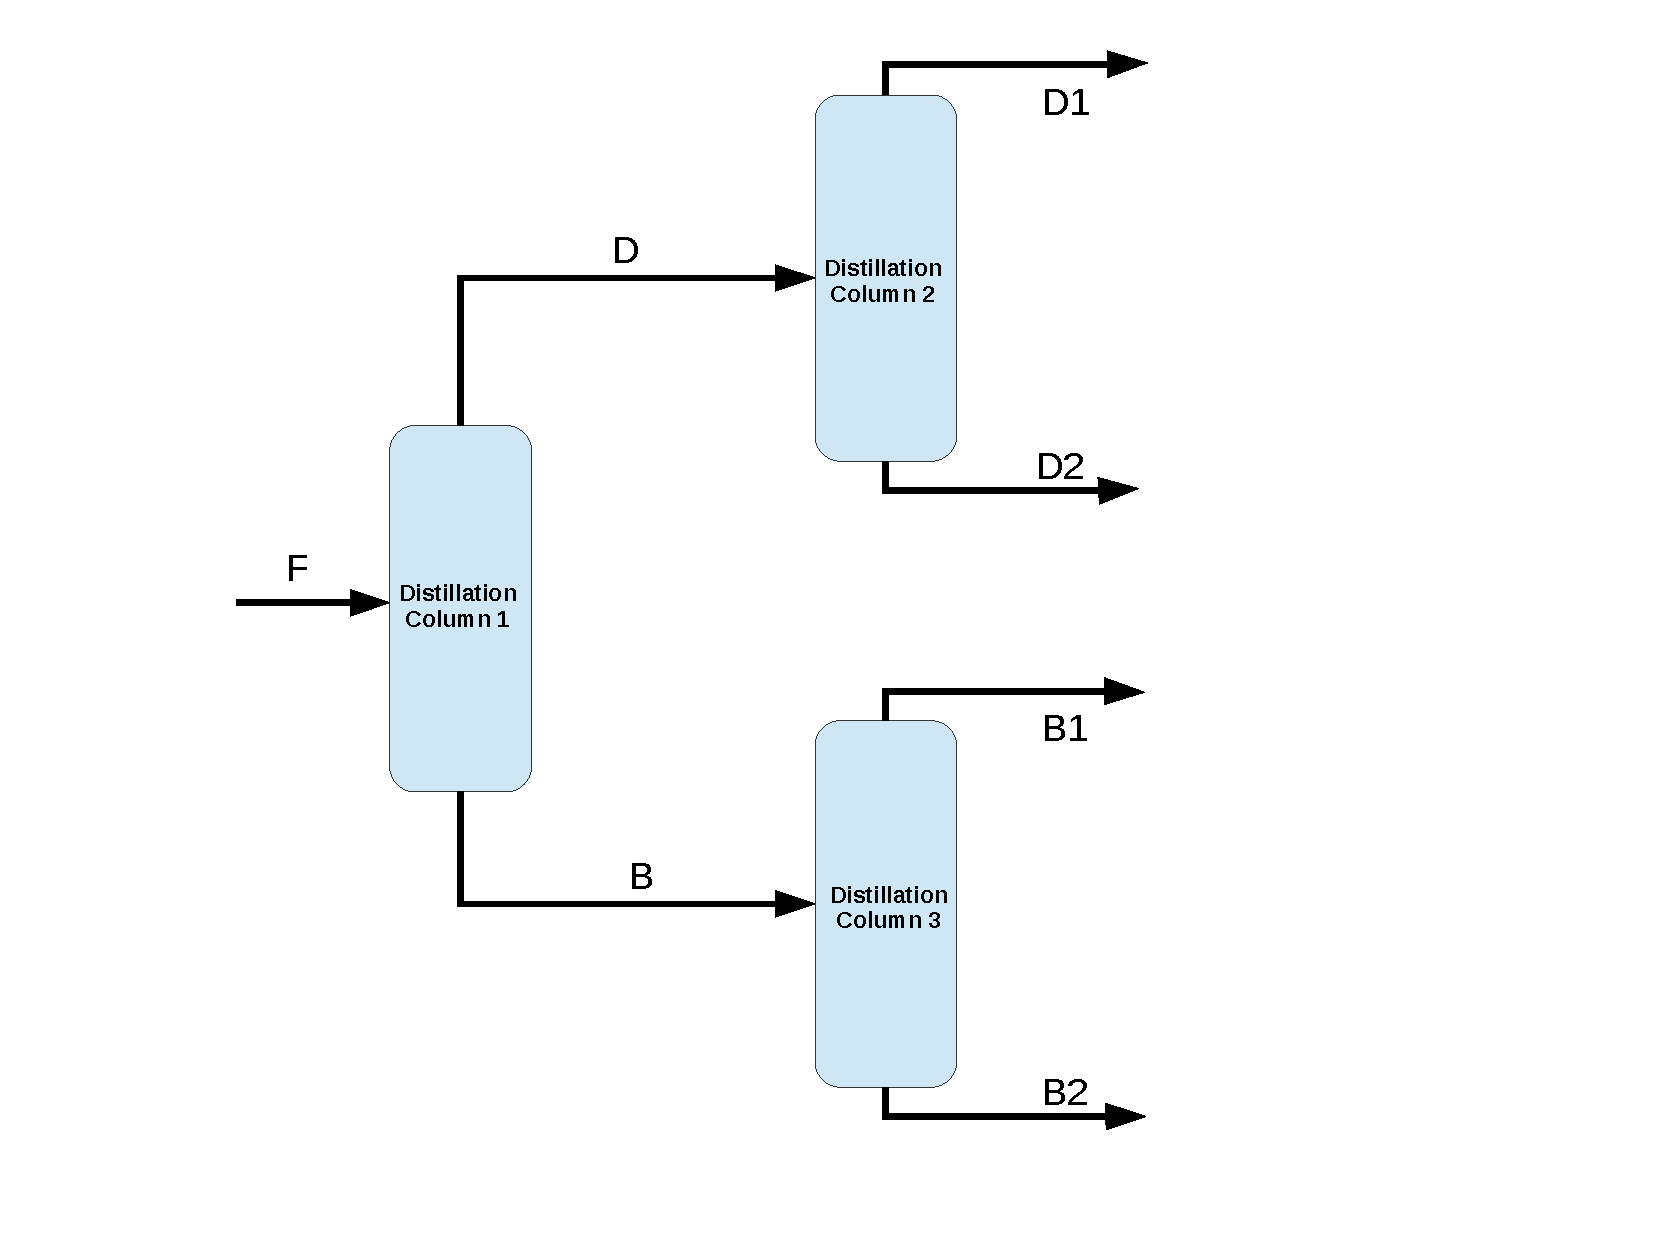
\includegraphics[width=15.cm,height=10.cm,clip]{./Pics/Practical_Distillation.pdf}
\caption{Distillation columns. }
\label{distillationcolumn}
\end{center}
\end{figure}

{\bf Write a Matlab code that calculates the mass balance of the distillation system and,}
\begin{enumerate}[label=\bfseries Task \arabic*]
\item Calculate molar flow rates (in gmol.s$^{-1}$) of streams $D1$, $D2$, $B1$ and $B2$;\hfill{\bf[15 Marks]}
\item Calculate molar flow rates (in gmol.s$^{-1}$) and compositions of streams $D$ and $B$.\hfill{\bf[15 Marks]}
\end{enumerate}

\end{enumerate}
\clearpage

{\bf Deliverables:}
\begin{itemize}
\item Write a report containing a brief introduction of EOS and a summary of your results (incl. figures displaying the data), findings along with concluding remarks and {\underline Matlab codes} used in your calculations. 
%
\item {\bf Prepare the report as \underline{PDF file} and submit it through {\it Turnitin} (with the appropriate plagiarism cover sheet) by Sunday, November 08$^{th}$ 2015, 23:59 at the latest.}
%
\item Feedback will be provided on November 30$^{th}$ 2015.
%
\item Penalties for late or non-submission are as follows:
\begin{enumerate}%[(a)]
\item Up to one week late, 2 CGS points deducted;
\item Up to two weeks late, 3 CGS point deducted;
\item More than two weeks late no marks awarded.
\end{enumerate}
If late or non-submission is due to medical or other circumstances out with your control you must submit a medical certificate or other formal evidence to the PGT Office as soon as is practicable but no later than the end of Revision Week.


\item Note that the submitted work is part of the continuous assessment which will contribute 20$\%$ to your EX3029 mark.

\end{itemize}

%\end{enumerate}


\clearpage

%{
%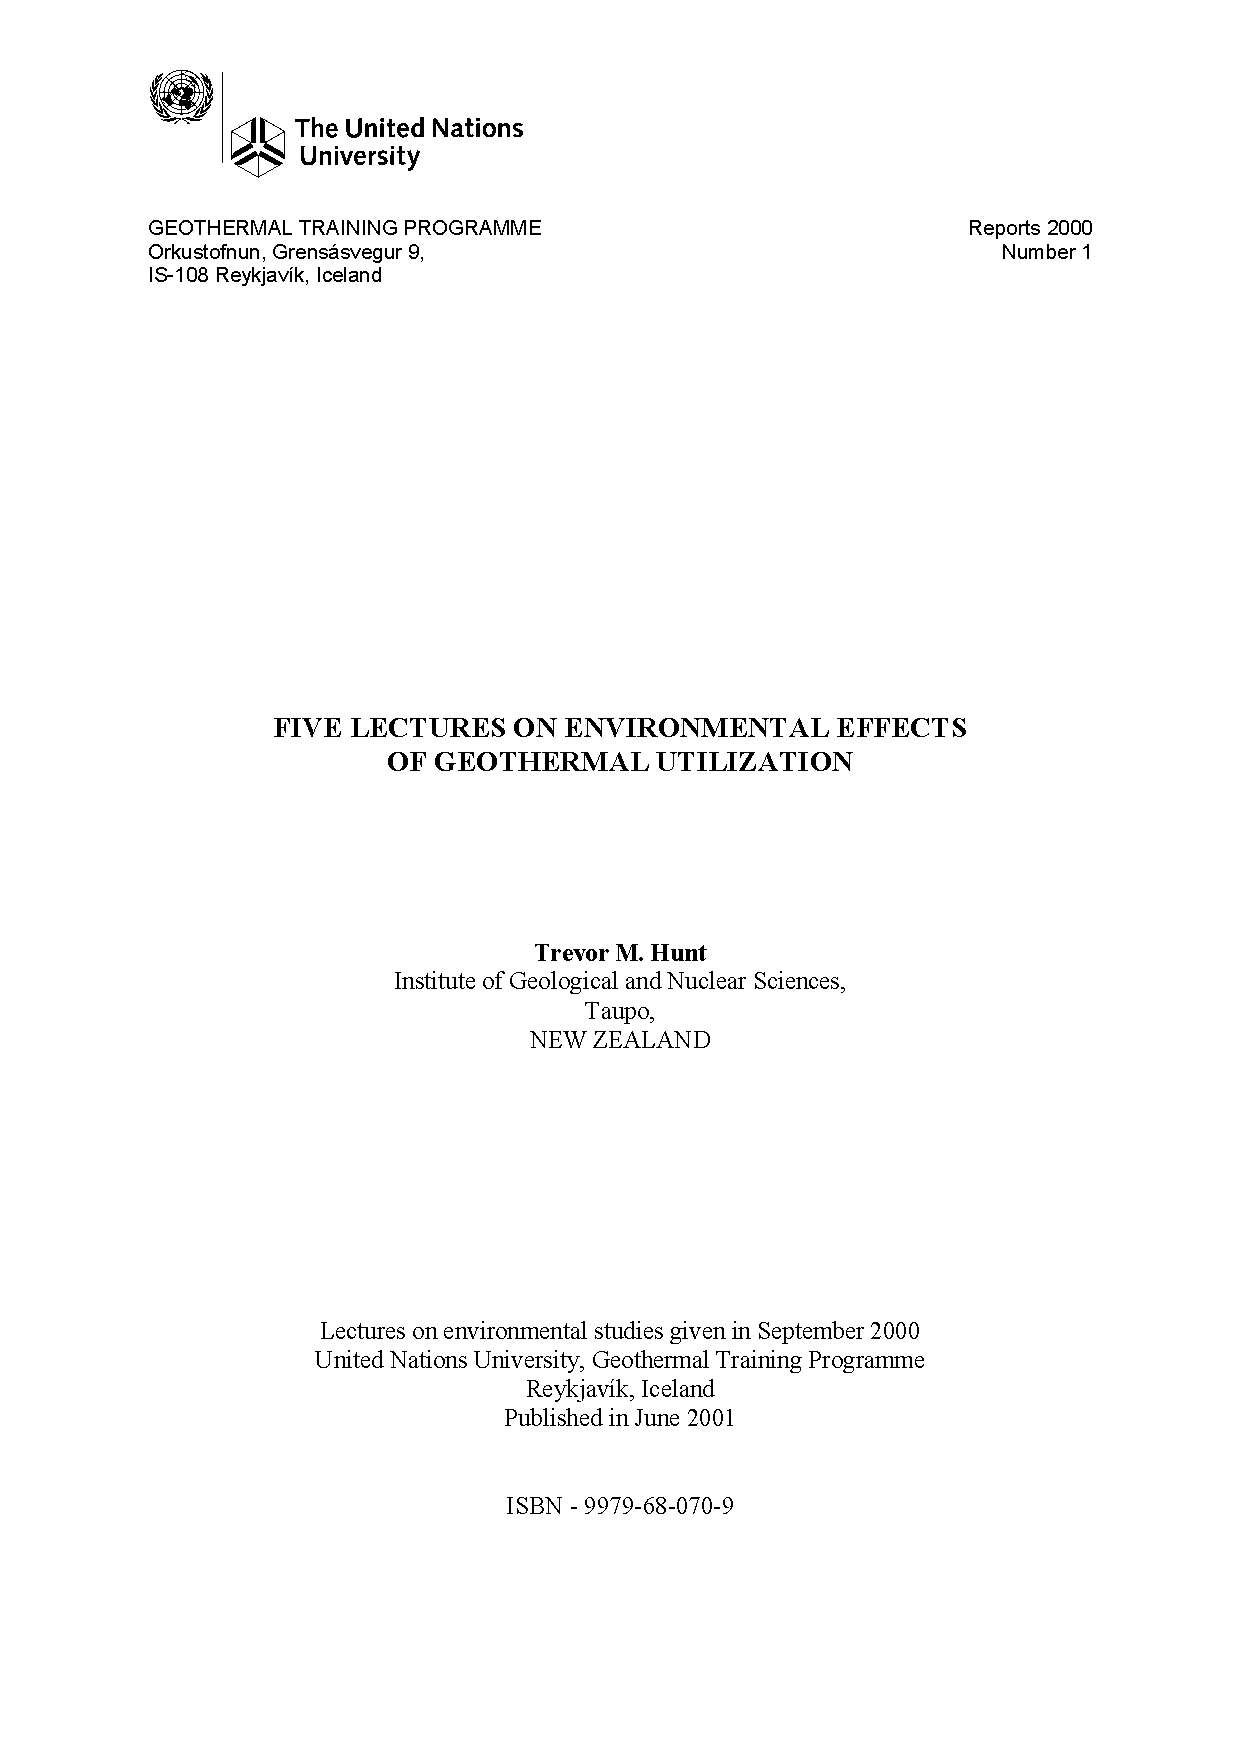
\includepdf[pages=-,fitpaper, angle=0]{./HuntSelect.pdf}
%}

\end{document}
